\section{DynNode Class Reference}
\label{classDynNode}\index{DynNode@{DynNode}}
node having conditional forward time belief information  


{\tt \#include $<$node.h$>$}

Inheritance diagram for DynNode::\begin{figure}[H]
\begin{center}
\leavevmode
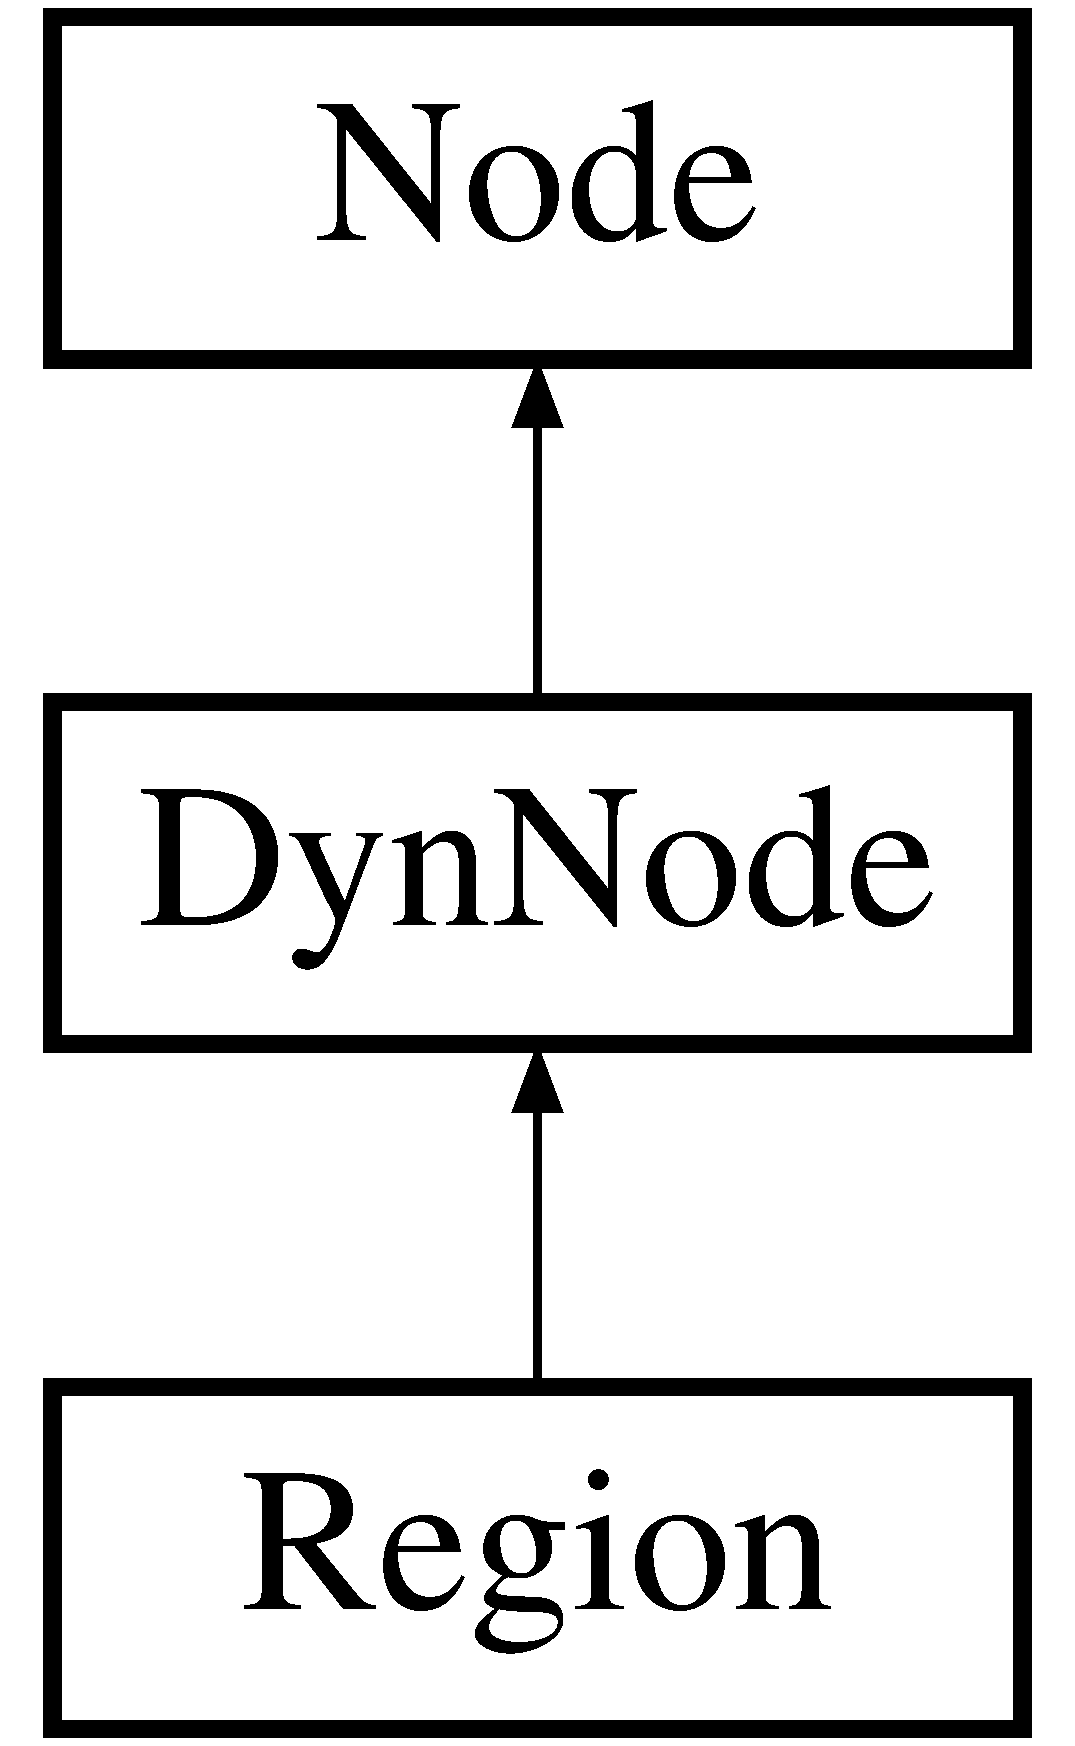
\includegraphics[height=3cm]{classDynNode}
\end{center}
\end{figure}
\subsection*{Public Member Functions}
\begin{CompactItemize}
\item 
{\bf DynNode} ()
\item 
void {\bf setConditionalBelief} ({\bf ConditionalBelief} $\ast$c)
\item 
{\bf DynNode} (string s, int {\bf numVar}, {\bf Belief} $\ast$bp=0, {\bf ConditionalBelief} $\ast$cbp=0, int \_\-type=-1)
\item 
{\bf ConditionalBelief} $\ast$ {\bf getConditionalBeliefPtr} ()
\item 
{\bf $\sim$DynNode} ()
\end{CompactItemize}
\subsection*{Private Attributes}
\begin{CompactItemize}
\item 
{\bf ConditionalBelief} $\ast$ {\bf cPtr}
\begin{CompactList}\small\item\em set of conditional beliefs about next state given current state \item\end{CompactList}\end{CompactItemize}
\subsection*{Friends}
\begin{CompactItemize}
\item 
ostream \& {\bf operator$<$$<$} (ostream \&os, {\bf DynNode} \&dn)
\end{CompactItemize}


\subsection{Detailed Description}
node having conditional forward time belief information 



\subsection{Constructor \& Destructor Documentation}
\index{DynNode@{DynNode}!DynNode@{DynNode}}
\index{DynNode@{DynNode}!DynNode@{DynNode}}
\subsubsection{\setlength{\rightskip}{0pt plus 5cm}DynNode::DynNode ()\hspace{0.3cm}{\tt  [inline]}}\label{classDynNode_f6e18d6646c290d1cc617e7f97837607}


\index{DynNode@{DynNode}!DynNode@{DynNode}}
\index{DynNode@{DynNode}!DynNode@{DynNode}}
\subsubsection{\setlength{\rightskip}{0pt plus 5cm}DynNode::DynNode (string {\em s}, int {\em numVar}, {\bf Belief} $\ast$ {\em bp} = {\tt 0}, {\bf ConditionalBelief} $\ast$ {\em cbp} = {\tt 0}, int {\em \_\-type} = {\tt -1})}\label{classDynNode_06541a46e4f4fc4db612917774e02a85}


\index{DynNode@{DynNode}!~DynNode@{$\sim$DynNode}}
\index{~DynNode@{$\sim$DynNode}!DynNode@{DynNode}}
\subsubsection{\setlength{\rightskip}{0pt plus 5cm}DynNode::$\sim$DynNode ()\hspace{0.3cm}{\tt  [inline]}}\label{classDynNode_be9a7aa589d8a07b52449724a9ca6240}




\subsection{Member Function Documentation}
\index{DynNode@{DynNode}!setConditionalBelief@{setConditionalBelief}}
\index{setConditionalBelief@{setConditionalBelief}!DynNode@{DynNode}}
\subsubsection{\setlength{\rightskip}{0pt plus 5cm}void DynNode::setConditionalBelief ({\bf ConditionalBelief} $\ast$ {\em c})\hspace{0.3cm}{\tt  [inline]}}\label{classDynNode_902d5999f06d232efba16c77b7366809}


\index{DynNode@{DynNode}!getConditionalBeliefPtr@{getConditionalBeliefPtr}}
\index{getConditionalBeliefPtr@{getConditionalBeliefPtr}!DynNode@{DynNode}}
\subsubsection{\setlength{\rightskip}{0pt plus 5cm}{\bf ConditionalBelief}$\ast$ DynNode::getConditionalBeliefPtr ()\hspace{0.3cm}{\tt  [inline]}}\label{classDynNode_adf2e00588988f9705de42c4c2930918}




\subsection{Friends And Related Function Documentation}
\index{DynNode@{DynNode}!operator<<@{operator$<$$<$}}
\index{operator<<@{operator$<$$<$}!DynNode@{DynNode}}
\subsubsection{\setlength{\rightskip}{0pt plus 5cm}ostream\& operator$<$$<$ (ostream \& {\em os}, {\bf DynNode} \& {\em dn})\hspace{0.3cm}{\tt  [friend]}}\label{classDynNode_ce217a788f52579d20aeabc6ef30650e}




\subsection{Member Data Documentation}
\index{DynNode@{DynNode}!cPtr@{cPtr}}
\index{cPtr@{cPtr}!DynNode@{DynNode}}
\subsubsection{\setlength{\rightskip}{0pt plus 5cm}{\bf ConditionalBelief}$\ast$ {\bf DynNode::cPtr}\hspace{0.3cm}{\tt  [private]}}\label{classDynNode_03326c806301531f149a01c9291245a9}


set of conditional beliefs about next state given current state 



The documentation for this class was generated from the following files:\begin{CompactItemize}
\item 
inc/{\bf node.h}\item 
src/{\bf node.cpp}\end{CompactItemize}
